% Chapter Template

\chapter{Model Transformation} % Main chapter title

\label{Chapte3} % Change X to a consecutive number; for referencing this chapter elsewhere, use \ref{ChapterX}

\lhead{Chapter 3. \emph{Model Transformation}} % Change X to a consecutive number; this is for the header on each page - perhaps a shortened title

In this chapter we will describe what model transformations is and also write
about the different types of model transformation. 
%----------------------------------------------------------------------------------------
%	SECTION 1
%----------------------------------------------------------------------------------------

\section{What is model transformation?}

Transformation is a fundamental theme in computer science and software
engineering. Whenever a computer starts up, transformation of computer systems
and computer programs happens frequently. Take a compiler for instance, it plays
a vital part of a computers internal infrastructure. A compiler is a computer
program that translates source code written in a high-level programming
language into lower level language, such as an assembly language or machine
code. This means that a computer program written in a general-purpose
programming language, such as Java or C++ would be useless without a compiler,
since the computer's central processing unit (CPU) depends on machine code to be
able to execute a set of instructions. But also computation of primitive data
values and performing operations on data structures such as lists can also be
viewed as data transformations. When a programming language provides a way
to type these data values or data structures, then a compiler or interpreter can
apply operations to the data accordingly to the type. But when we talk about
data representing software artifacts such as a data schema, programs or models,
then transformation approaches 

Machine code or machine language is a set of instructions executed directly by a
computer's central processing unit (CPU). Each instruction performs a very
specific task, such as a load, a jump, or an ALU operation on a unit of data in
a CPU register or memory. Every program directly executed by a CPU is made up
of a series of such instructions.

%-----------------------------------
%	SUBSECTION 1
%-----------------------------------
\subsection{Basic concepts of model transformation}

The basic concept of model transformations is to do changes to a model. 

A model transformation is when we change an instance of a source metamodel to an
instance that conforms to the target metamodel. We can distinguish these operations into either endogenous or exogenous model transformations. In an
endogenous model transformation we take one model expressed in a language and
produce a model expressed in the same language.
While an exogenous model transformation start with a model expressed in one
modelling language and translate this into a model expressed in another
modelling language. It is essential that these models are consistent. This is
obtained through the use of metamodels. A metamodel is a description of a
modelling language, where it defines elements that are used in the model.
A model transformation can produce two different kind of output models. The
first one is code generation, often referred to Model to Text(M2T)
transformation, and it takes one model and produces implementation code. This
is convenient if for example a software engineer wants to produce source code
from a given model. asdsd
\begin{figure}[H]
  \centering
    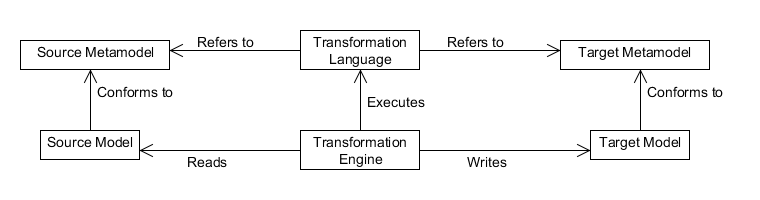
\includegraphics[scale=0.5]{./Figures/BasicTransformation.png}
    \rule{35em}{0.5pt}
  \caption[Basic Model Transformation]
  				{The basic concepts behind a model
  transformation.}
  \label{fig:BasicTransformation}
\end{figure}

%-----------------------------------
%	SUBSECTION 2
%-----------------------------------

\subsection{Classification of a model transformation}

\begin{figure}[H]
  \centering
    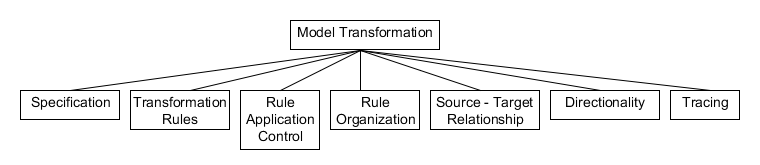
\includegraphics[scale=0.5]{./Figures/Model_Transformation_Survey.png}
    \rule{35em}{0.5pt}
  \caption[Domain Analysis of Model Transformations]
  				{A domain analysis of model transformations.}
  \label{fig:Model_Transformation_Survey}
\end{figure}

Domain-Specific Metamodelling Languages for Software Language Engineering
%----------------------------------------------------------------------------------------
%	SECTION 2
%----------------------------------------------------------------------------------------

\section{Graph Transformation} 
\noindent One approach to model transformations is by graph transformations,
also referred to as graph rewriting. Graph rewriting can be implemented with
an algebraic approach, which is based on category theory\cite{Barr1990}.

\begin{figure}[H]
	\centering
	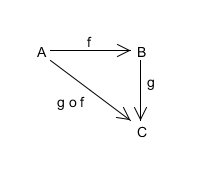
\includegraphics[scale=0.7]{./Figures/categoryTheory.png}
	\caption{Collection of objects A,B and C.}
	\label{fig:categoryTheory}
\end{figure}


In category theory there are a collection of objects and arrows. These arrows
are also called morphisms. In figure~\ref{fig:categoryTheory} we have a
collection of objects A, B and C and morphisms f, g and g $\circ$ f. And for the
purpose of this paper, the collection of objects are graphs and the arrows are
graph morphisms. This is also very typical when writing papers to explain the
concepts of graph transformations, where these objects are represented as
graphs, and arrows are represented as morphisms. Category theory can then be
used to formalize the concepts at a high level of abstraction.

\subsection{The Algebraic Approach}
\noindent This approach are based on the concepts of composing graphs, modelled
by pushouts of graphs and graph morphisms. This pushout approach comes in
different variants, and we will look at two of these, namely the
double-pushout (DPO) approach and the single pushout (SPO)
approach\cite{Loewe1997,Ehrig1997}.

\indent Historically, the first of the algebraic approaches to graph
transformations, the double-pushout, was first introduced at the Technical
University of Berlin in the early seventies by H. Ehrig, M. Pfender and H.J.
Schneider\cite{INSPEC:606170}. They tried to generalize Chromsky grammars from
strings to graphs. This allowed to define a graph rewriting step by the use of
two gluing constructions. And by applying a graph rewriting step for the
double-pushout approach is a pair of morphisms in the category of graphs where
the arrows represents total graph morphisms, \linebreak\mbox{L $\longleftarrow$
\ K $\longrightarrow$ R}. This is true for each application rule in a graph
transformation for the double-pushout approach. Where the graph K represents the
common part and the two morphisms \mbox{L $\longleftarrow$ \ K} and \mbox{K
$\longrightarrow$ R} use the algebraic construction, pushout to apply an
application rule for a rewriting step. Hence the name double pushout and the use
of two rewriting conditions.

\subsection{Productions}
\noindent For a transformation language to be able to execute graph
transformations a set of application rules needs to be defined. Through these
rules, a transformation interpreter can act accordingly. These rules are often
referred to as Productions. For graph transformations, there can be an arbitrary
number of rules. Its truly up to the users how they want to translate a
language and how many rules that is needed to acquire this. Each rule consists
of a left hand side (LHS) and a right hand side (RHS), also often referred to as
pattern graph and replacement graph. The pattern graph represents a subgraph of
the model that is going to be translated, namely the host graph. For these
productions to execute, there has to be some control mechanism, namely the
transformation unit.


\subsection{Transformation Units}
\noindent In graph transformation, there has to be a control mechanism that
administrates these productions. These control mechanisms are also called
transformation units. These units controls the order that the transformation
rules are executed. The most basic transformation unit is a rule itself which
corresponds to a single application of that rule. But in most cases, a
transformation unit will have to control several rule applications. 

\subsection{A Direct Derivation}
\noindent The basic idea for graph transformation for both the double-pushout
approach and the single pushout approach is to apply an application rule
\mbox{r: L $\longrightarrow$ R}. Where the rule represents a single rewriting
step for graph transformations and L represents the left hand side of the rule and R
represents the right hand side of the rule.

\begin{figure}[H]
	\centering
	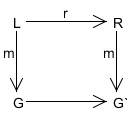
\includegraphics[scale=0.7]{./Figures/GraphTransformationGeneral.png}
	\caption{The basic idea for graph transformation by applying a rule r.}
	\label{fig:GraphTransformationGeneral}
\end{figure}

For a production rule r, \mbox{G$\xrightarrow{r,m}$G'} indicates a direct
derivation to a derived graph G'. In
figure~\ref{fig:GraphTransformationGeneral}, the graph G' is created by
applying a single pushout for a transformatin rule r. If there is a match m of
nodes and arrows for a subgraph L in a host graph G, then this indicates a
graph homomorphism, mapping elements from the subgraph to the host graph in
such a way that the graphical structure in G is preserved. For each rule r,
there are some algebraic approaches to how we can achieve G'. At this moment
there are four approaches, the double-pushout approach (DPO) \cite{Loewe1997}, the
single-pushout approach (SPO) \cite{Ehrig1997}, the sesqui-pushout and the
pullback approach. Where the two most common approaches used in graph
transformation tools are the DPO and the SPO approach. There is one major
aspect that separate these two approaches, and that is that the DPO approach
has an application condition.

\begin{figure}[H]
	\centering
	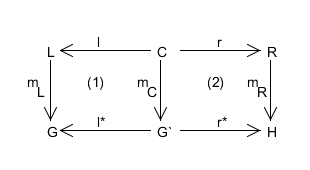
\includegraphics[scale=0.7]{./Figures/DPO.png}
	\caption{Principles behind the double pushout approach.}
	\label{fig:DPO}
\end{figure}

\noindent This application condition, named the gluing condition\cite{Loewe1997}
consists of two parts. Namely the dangling condition and identification
condition. From figure~\ref{fig:DPO}, the dangling condition requires that if
the transformation rule p specifies the deletion of a node in G, then it must also
specify the deletion of all incoming and outgoing edges of this node in G. By
applying this condition, we can be sure that there are no dangling edges after
deleting a node in G. The identification condition requires that every element
of G that should be deleted by applying a transformation rule p is only present
once in L for each transformation rule p. 

A single transformation rule p in the DPO approach is given by a pair of graph
homomorphisms from a common graph C. This common graph C is formed by taking
elements that are present in both L (LHS) and R (LHS) of a transformation rule
p. The graph G' are created from the graph G, by deleting all elements that is
matched from the pattern graph L, but none in C. To avoid dangling edges,
the gluing condition must be satisfied before deleting these elements. This is
the first part (1) of the DPO approach, namely the deletion of elements. The
second part (2) is insertion of elements. From here we create a graph H off all
nodes and arrows from the replacement graph R that is not presented in the
common graph C. The DPO approach has the possibility to preserve elements from
translating from the pattern graph L and the replacement graph R with the help
of a common graph C.

For the SPO approach on the other hand, deletion has priority over preservation.
Figure~\ref{fig:GraphTransformationGeneral} is a representation of the practices
of the SPO approach. Where nodes that are present in the pattern graph L but not
the replacement graph R are deleted. And the incoming and outgoing edges of the
deleted nodes that are not present in the replacement graph R is deleted.

Now that we have explained some aspects of Graph transformations, we can
describe the three different tools, where both AGG and Henshin is build around
the concepts of graph transformations explained in this section. 

